% Hlavicka pro protokoly z fyzikalniho praktika.
% Verze pro: LaTeX
% Verze hlavicky: 22. 2. 2007
% Autor: Ustav fyziky kondenzovanych latek
% Ke stazeni: www.physics.muni.cz/ufkl/Vyuka/
% Licence: volne k pouziti, nejlepe k vcasnemu odevzdani protokolu z Vaseho mereni.

\documentclass[a4paper,11pt]{article}

% Kodovani (cestiny) v dokumentu: utf-8
%\usepackage[cp1250]{inputenc}	% Omezena stredoevropska kodova stranka, pouze MSW.
\usepackage[utf8]{inputenc}	% Doporucujeme pouzivat UTF-8 (unicode).

%%% Nemente:
\usepackage[margin=2cm]{geometry}
\newtoks\jmenopraktika \newtoks\jmeno \newtoks\datum
\newtoks\obor \newtoks\skupina \newtoks\rocnik \newtoks\semestr
\newtoks\cisloulohy \newtoks\jmenoulohy
\newtoks\tlak \newtoks\teplota \newtoks\vlhkost
\usepackage{amsmath}
\usepackage{mathtools}
\usepackage{graphicx}
\usepackage{multirow}
\graphicspath{ {./images/} }
%%% Nemente - konec.


%%%%%%%%%%% Doplnte pozadovane polozky:

\jmenopraktika={Fyzikální praktikum 2}  % nahradte jmenem vaseho predmetu
\jmeno={Artem Gorodilov}            % nahradte jmenem mericiho
\datum={21. ~prosince  2023}        % nahradte datem mereni ulohy
\obor={Astrofyzika}                     % nahradte zkratkou vami studovaneho oboru
\skupina={Čt 8:00}            % nahradte dobou vyuky vasi seminarni skupiny
\rocnik={II}                  % nahradte rocnikem, ve kterem studujete
\semestr={I}                 % nahradte semestrem, ve kterem studujete

\cisloulohy={2}               % nahradte cislem merene ulohy
\jmenoulohy={Charakteristiky tranzistoru} % nahradte jmenem merene ulohy

\tlak={981}                   % nahradte tlakem pri mereni (v hPa)
\teplota={21.6}               % nahradte teplotou pri mereni (ve stupnich Celsia)
\vlhkost={49}               % nahradte vlhkosti vzduchu pri mereni (v %)

%%%%%%%%%%% Konec pozadovanych polozek.


%%%%%%%%%%% Uzitecne balicky:
\usepackage[czech]{babel}
\usepackage{graphicx}
\usepackage{amsmath}
\usepackage{xspace}
\usepackage{url}
\usepackage{indentfirst}
\usepackage{listings}
\usepackage{subcaption}
\usepackage{caption}
\usepackage{tabularx}
\usepackage[labelformat=parens,labelsep=quad,skip=3pt]{caption}

%%%%%% Zamezeni parchantu:
\widowpenalty 10000 \clubpenalty 10000 \displaywidowpenalty 10000
%%%%%% Parametry pro moznost vsazeni vetsiho poctu obrazku na stranku
\setcounter{topnumber}{3}	  % max. pocet floatu nahore (specifikace t)
\setcounter{bottomnumber}{3}	  % max. pocet floatu dole (specifikace b)
\setcounter{totalnumber}{6}	  % max. pocet floatu na strance celkem
\renewcommand\topfraction{0.9}	  % max podil stranky pro floaty nahore
\renewcommand\bottomfraction{0.9} % max podil stranky pro floaty dole
\renewcommand\textfraction{0.1}	  % min podil stranky, ktery musi obsahovat text
\intextsep=8mm \textfloatsep=8mm  %\intextsep pro ulozeni [h] floatu a \textfloatsep pro [b] or [t]

% Tecky za cisly sekci:
\renewcommand{\thesection}{\arabic{section}.}
\renewcommand{\thesubsection}{\thesection\arabic{subsection}.}
% Jednopismenna mezera mezi cislem a nazvem kapitoly:
\makeatletter \def\@seccntformat#1{\csname the#1\endcsname\hspace{1ex}} \makeatother

\begin{document}

\thispagestyle{empty}

{
\begin{center}
\sf 
{\Large Ústav fyzikální elektroniky PřF MU} \\
\bigskip
{\huge \bfseries FYZIKÁLNÍ PRAKTIKUM} \\
\bigskip
{\Large \the\jmenopraktika}
\end{center}

\bigskip

\sf
\noindent
\setlength{\arrayrulewidth}{1pt}
\begin{tabular*}{\textwidth}{@{\extracolsep{\fill}} l l}
\large {\bfseries Zpracoval:}  \the\jmeno & \large  {\bfseries Naměřeno:} \the\datum\\[2mm]
\large  {\bfseries Obor:} \the\obor  \hspace{40mm}  {\bfseries Skupina:} \the\skupina %
%{\bfseries Ročník:} \the\rocnik \hspace{5mm} {\bfseries Semestr:} \the\semestr  
&\large {\bfseries Testováno:}\\
\\
\hline
\end{tabular*}
}

\bigskip

{
\sf
\noindent \begin{tabular}{p{3cm} p{0.6\textwidth}}
\Large  Úloha č. {\bfseries \the\cisloulohy:} \par
\smallskip
$T=\the\teplota$~$^\circ$C \par
$p=\the\tlak$~hPa \par
$\varphi=\the\vlhkost$~\%
&\Large \bfseries \the\jmenoulohy  \\[2mm]
\end{tabular}
}

\vskip1cm
    \begin{minipage}[t]{0.5\textwidth} 
        \section{Zadání}
            Určit charakteristiku tranzistoru.
            \par Použít tranzistor jako napěťový zesilovač.
        \section{Teorie}
            \subsection{Charakteristiky tranzistoru}
                Tranzistor představuje nelineární rezistivní komponentu, což implikuje, že nepodléhá ohmovu zákonu. Jeho výstupní vlastnosti jsou závislé na napětí přes hradlo. Dále je charakteristické pro tranzistory, že mohou fungovat jako zesilovače proudu nebo napětí v určitých elektrických obvodech. V tomto příkladu se zaměříme na unipolární tranzistor, což značí, že pro vodivost jsou zodpovědné buď elektrony nebo díry. Tyto nábojové nosiče se vyskytují v oblasti nazývané kanál, který je vybaven dvěma elektrickými kontakty, označenými jako source $S$ a drain $D$. Proud procházející kanálem je ovlivněn napětím mezi source $S$ a izolovanou elektrodou ($p-n$ přechod nebo oxidová vrstva), která se nazývá gate $G$.
                \par Při využití tranzistoru jako zesilovače se zaměřím na specifický pracovní bod tranzistoru, určený konstantním napětím na drainu a hradle. Tento bod je lokalizován v místě, kde se protínají křivky převodní a výstupní charakteristiky pro zvolené hodnoty napětí.
                \par S nastaveným pracovním bodem je možné definovat klíčové parametry tranzistoru v tomto bodě,
    \end{minipage}
    \hspace{10pt}
    \begin{minipage}[t]{0.5\textwidth} 
                jako jsou strmost $S$, vnitřní odpor $R_i$ a zesilovací faktor $\mu$, které jsou určeny specifickými vztahy:
                \begin{equation}
                    S = \left\frac{\partial I_D}{\partial U_G}\right\vert_{U_D=const}
                \end{equation}
                kde $I_D$ je proud na drainu a $U_G$ je napětí na gate.
                \begin{equation}
                    R_i = \left\frac{\partial U_D}{\partial I_D}\right\vert_{U_G=const}
                \end{equation}
                kde $U_D$ je napětí na drainu.
                \begin{equation}
                    \mu = \left\frac{\partial U_D}{\partial U_G}\right\vert_{I_D=const}
                \end{equation}
                Strmost $S$, anebo $R_i$, je možné vypočítat jako směrnici tečny k převodní nebo výstupní charakteristice tranzistoru v zvoleném pracovním bodě. Zesilovací činitel $\mu$ pak lze určit pomocí Barkhausenovy rovnice.
                \begin{equation}
                    SR_i\frac{1}{\mu} = 1 ~~\longrightarrow~~ \mu = SR_i
                \end{equation}
                Při měřeních bylo použito následující schéma:
                \vspace{10pt}
                \par \centering
                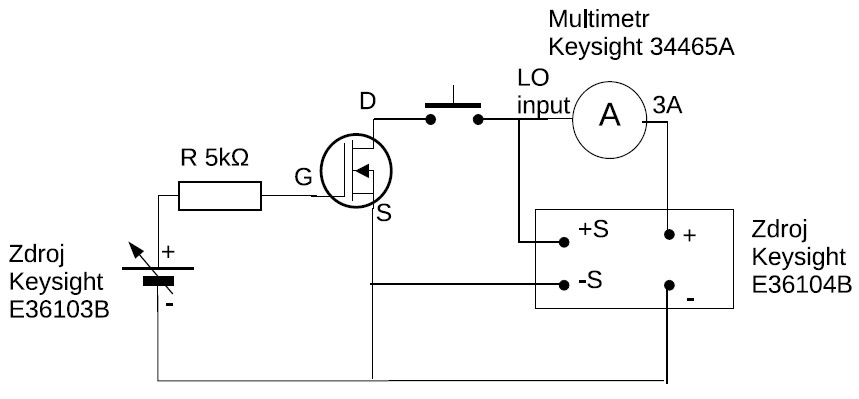
\includegraphics[scale=0.35]{char}
                \captionsetup{justification=centering, font=footnotesize}
                \captionof{figure}{Schéma zapojení pro měření charakteristik tranzistoru.}
                \label{fig:char}
                \raggedright
    \end{minipage}
\newpage
    \begin{minipage}[t]{0.5\textwidth} 
            \subsection{Tranzistor jako zesilovač napětí}
                Chcete-li tranzistor použít jako zesilovač, musí být zapojen podle obrázku (2). 
                \vspace{10pt}
                \par \centering
                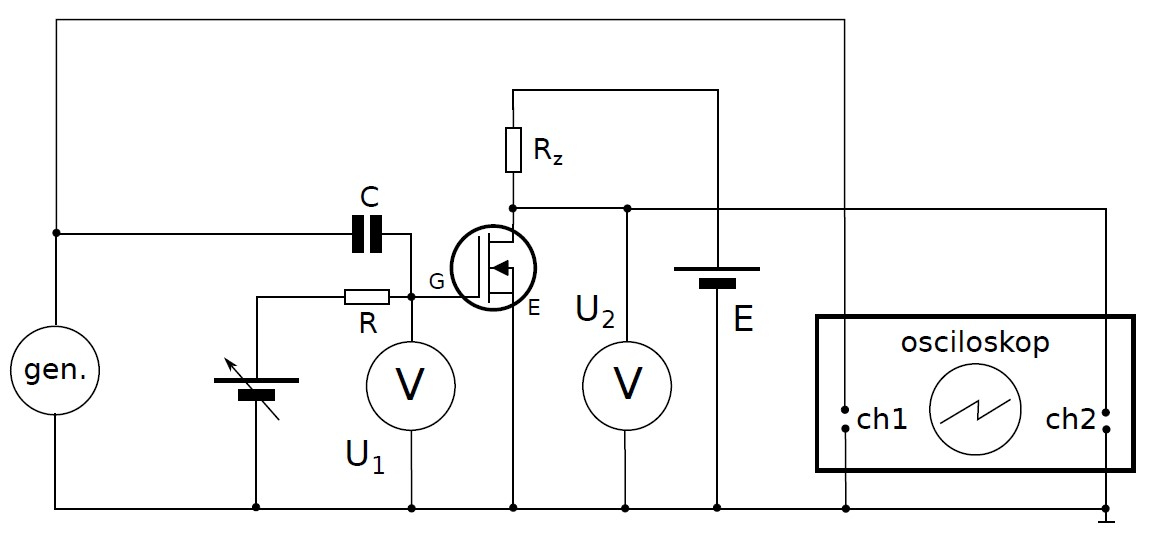
\includegraphics[scale=0.25]{zas}
                \captionsetup{justification=centering, font=footnotesize}
                \captionof{figure}{Schéma zapojení pro použití tranzistoru jako zesilovače napětí.}
                \label{fig:zas}
                \raggedright
                \vspace{10pt}
                Toto zapojení lze chápat jako napěťový dělič, kde součet napětí na tranzistoru $U_D$ a na zátěžovém odporu $R_Z$ odpovídá napětí $E$. Zvýšení napětí na $G$ sníží odpor tranzistoru, což vede k poklesu napětí na $D$ a následně k zvýšení napěťového úbytku na zátěžovém odporu. Změna napětí na $D$ je mnohonásobně větší než změna na $G$, což vede k napěťovému zesílení. 
                \par Zesílení tranzistorového zesilovače $A_V$ je definováno určitým vztahem:
                \begin{equation}
                    A_V = \frac{SR_Z}{1+\frac{R_Z}{R_i}}
                \end{equation}
                Zatěžovací odpor $R_Z$ tim padem se spočítá jako:
                \begin{equation}
                    R_Z = \frac{E - U_{D0}}{I_{D0}}
                \end{equation}
                kde $E$ je napětí na zdroji, $U_{D0}$ je napětí na drainu a $I_{D0}$ je proud na drainu v pracovním bodě.
                \par Zesílení $A_G$ lze dále definovat graficky. Tento způsob je naznačen na obrázku (3) a je znázorněn následujícím vzorcem: 
                \begin{equation}
                    A_G = \frac{\Delta U_{D}}{\Delta U_{G}}
                \end{equation}
                \par \centering
                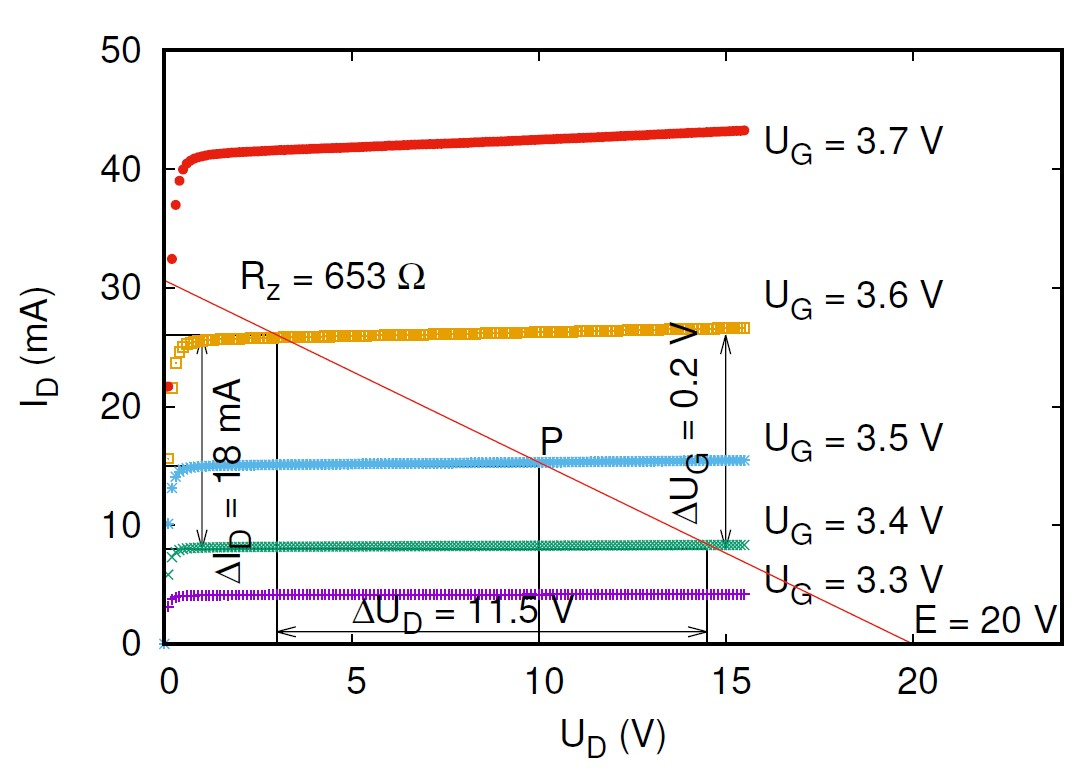
\includegraphics[scale=0.29]{zas2}
                \captionsetup{justification=centering, font=footnotesize}
                \captionof{figure}{Výstupní charakteristika tranzistoru. Zesílení $A_G$ je definováno jako poměr změny napětí na $D$ a $G$.}
                \label{fig:zas2}
                \raggedright
                \vspace{10pt}
    \end{minipage}
    \hspace{10pt}
    \begin{minipage}[t]{0.5\textwidth} 
                Pro určení zesílení $A_M$ použiji dvoukanálový osciloskop, kterým změřím dvojnásobek amplitudy vstupního napětí $u_{m1}$ a amplitudu výstupního napětí $u_{m2}$. Zesílení následně vypočítám jako poměr výstupní amplitudy napětí ku vstupní amplitudě:
                \begin{equation}
                    A_M = \frac{u_{m2}}{u_{m1}}
                \end{equation}
        \section{Měření}  
            \subsection{Charakteristiky tranzistoru}
                Na začátku jsme nastavili napětí na drainu na hodnotu $U_D$ = 10 [V], poté jsme změřili napětí na gejtu $U_G$ a proud na drainu $I_D$, z čehož jsme vynesli převodní charakteristiku, která je vidět v grafu (4). 
                \vspace{10pt}
                \par \centering
                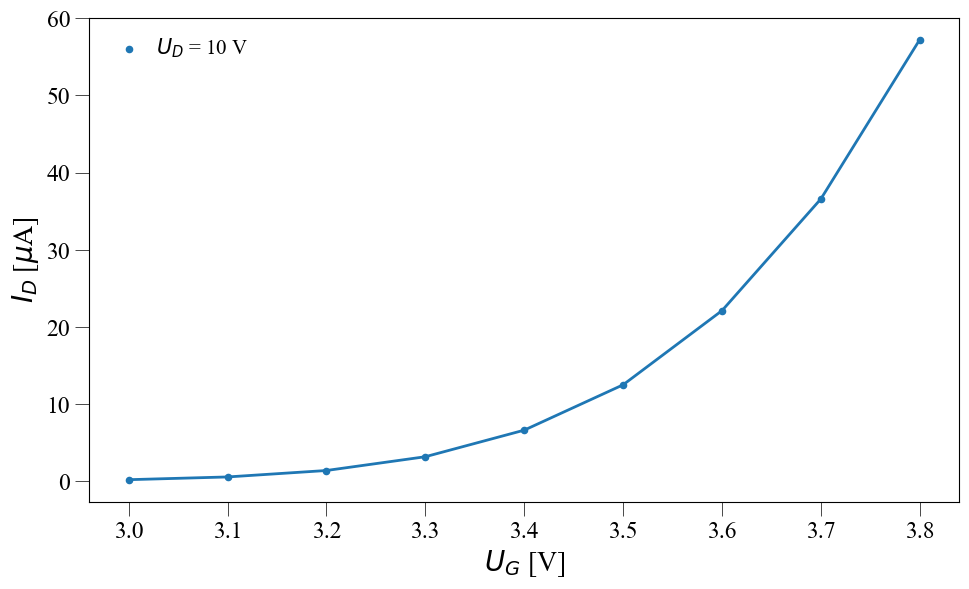
\includegraphics[scale=0.35]{prev_out}
                \captionsetup{justification=centering, font=footnotesize}
                \captionof{figure}{Převodní charakteristika tranzistoru.}
                \label{fig:prev_out}
                \raggedright
                \vspace{10pt}
                Poté jsme nastavili napětí na gejtu $U_G$ = 3.4 [V], načež jsme změřili napětí na dreinu $U_D$ a sílu proudu na dreinu $I_D$, z čehož jsme vynesli výstupní charakteristiku, která je vidět v grafu (5). 
                \vspace{10pt}
                \par \centering
                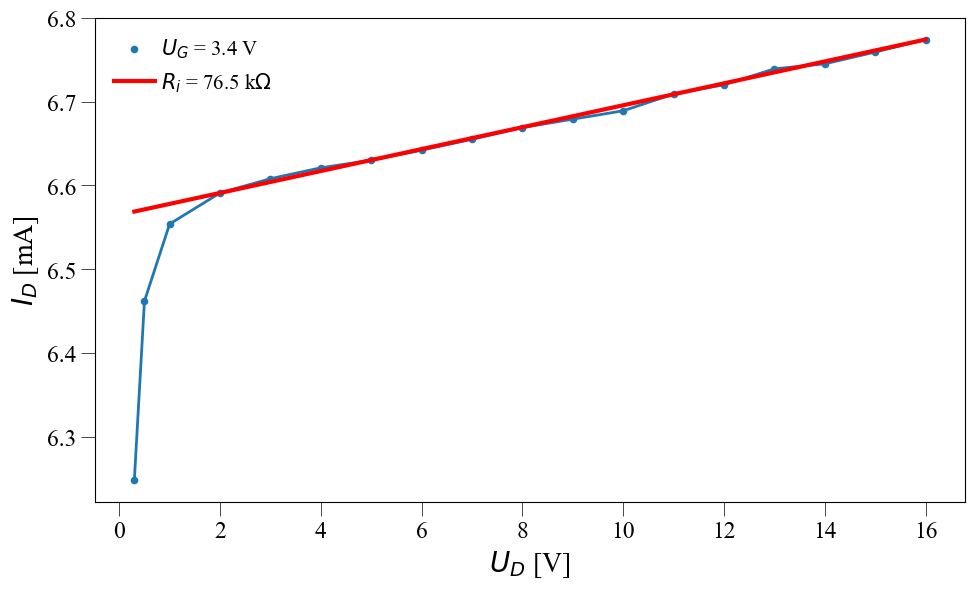
\includegraphics[scale=0.35]{vyst_out}
                \captionsetup{justification=centering, font=footnotesize}
                \captionof{figure}{Výstupní charakteristika tranzistoru.}
                \label{fig:vyst_out}
                \raggedright
                \vspace{10pt}
                \par Poté jsme změřili převodní charakteristiku pomocí počítače, hodnota $U_D$ zůstala 10 V. Pomocí počítače jsme změřili také výstupní charakteristiku, v tomto případě jsme nastavili hodnoty $U_G$ resp: 3.3 V, 3.4 V a 3.5 V. 
                \par Výsledky jsou znázorněny v grafu (6). 
    \end{minipage}
\newpage
                \begin{figure}[ht!]
                    \centering
                    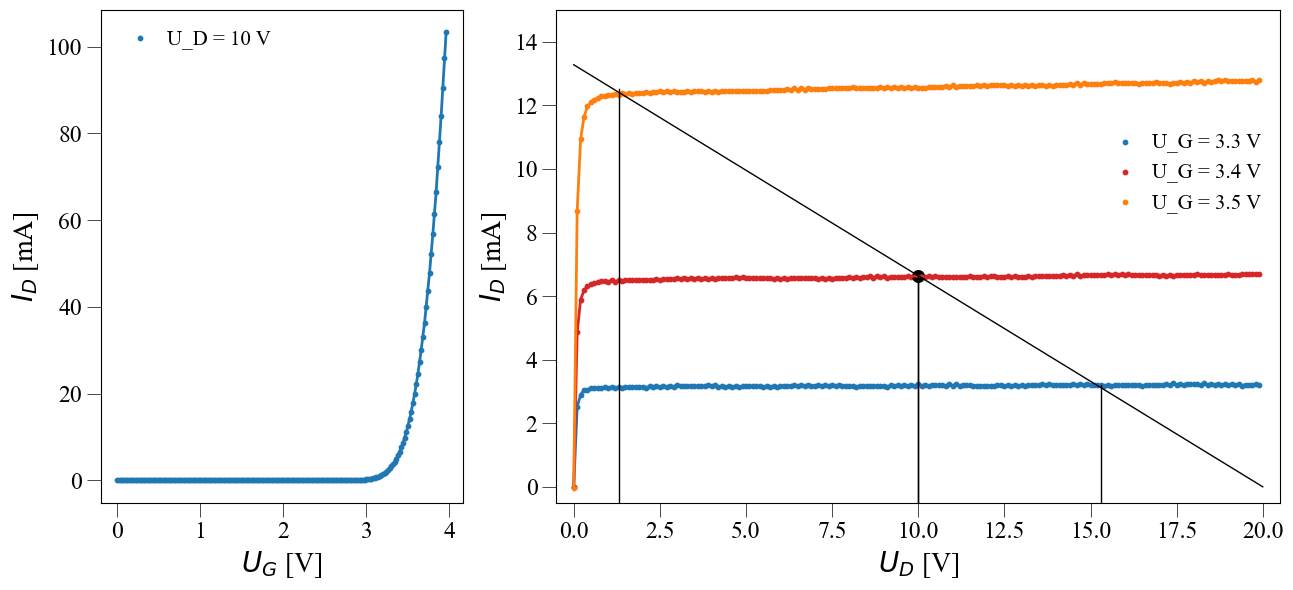
\includegraphics[scale=0.5]{pr_vs}
                    \captionsetup{justification=centering, font=footnotesize}
                    \captionof{figure}{Převodní (zleva) a výstupní (zprava) charakteristika tranzistoru.}
                    \label{fig:pr_vs}
                \end{figure}
    \begin{minipage}[t]{0.5\textwidth}
                Dále jsme definovali pracovní bod $P$ ($U_{D0}$ = 10 V, $U_{G0}$ = 3.4 V, $I_{D0}$ = 6.639 mA). Odtud najdeme Strmost $S$ a vnitřní odpor $R_i$ podle fomulí (1) a (2), přičemž najdeme derivaci v pracovním bodě $P$ pro převodní charakteristiku. Za tímto účelem byla funkce převodní charakteristiky interpolována a extrapolována pomocí knihovny $scipy~interp1d$.
                \begin{center}
                    $S$ = 24(3) [m$\Omega^{-1}$] \hspace{10pt} $R_i$ = 76.5(2) [k$\Omega$]
                \end{center}
                \par Zesílení $\mu$ jsme určili pomocí Barkhausenovy rovnice (4):
                \begin{center}
                    $\mu$ = 1.8(3)$\cdot$~10$^3$
                \end{center}
            \subsection{Tranzistor jako zesilovač napětí}
            Při použití tranzistoru jako napěťového zesilovače jsme při znalosti hodnot $U_{D0}$, $U_{G0}$ a $I_{D0}$ v našem pracovním bodě $P$ a při znalosti napětí $E$ = 20 V zjistili zatěžovací odpor $R_Z$ podle vzorce (6):
            \begin{center}
                $R_Z$ = 1506 [$\Omega$]
            \end{center}
            Proto při znalosti hodnot $S$ a $R_i$ vypočtených v předchozí části zjistíme hodnotu zesílení $A_V$ podle vzorce (5):
            \begin{center}
                $A_V$ = 35(5)
            \end{center}
            \par Zesílení $A_G$ jsme určili graficky podle vzorce (7). Výsledky jsou znázorněny v grafu (6):
            \begin{center}
                $\Delta U_D$ = 14 [V]
                \vspace{5pt}
                \par $\Delta U_G$ = 0.2 [V]
                \vspace{5pt}
                \par $A_G$ = 70
            \end{center}
    \end{minipage}
    \hspace{10pt}  
    \begin{minipage}[t]{0.5\textwidth} 
                Poté jsme změřili vstupní a výstupní hodnoty dvojnásobku amplitudy napětí $u_{m1}$ a $u_{m2}$, načež jsme pomocí vzorce (8) zjistili hodnoty $A_M$ pro každou z dvojic hodnot amplitudy. Výsledky jsou uvedeny v tabulce (1). 
                \vspace{10pt}
                \par \centering
                \begin{tabular}{|c|c|c|}
                    \hline
                    $u_{m1}$ [V] & $u_{m2}$ [V] & $A_M$ \\
                    \hline
                    0.0274 & 1.82 & 66.423358 \\
                    \hline
                    0.0728 & 4.88 & 67.032967 \\
                    \hline
                    0.1280 & 8.46 & 66.093750 \\
                    \hline
                    0.1600 & 10.80 & 67.500000 \\
                    \hline
                    0.2280 & 14.80 & 64.912281 \\  
                    \hline
/mnt/c/Users/shepo/Desktop/Учебные материалы/3rd semestr/fp2/Fyzikální praktikum 2 (Elektrické pole, můstkové metody měření odporu) (č 3)                \end{tabular}
                \captionsetup{justification=centering, font=footnotesize}
                \captionof{table}{Hodnoty $A_M$ pro každou z dvojic hodnot amplitud $u_{m1}$ a $u_{m2}$.}
                \vspace{10pt}
                \raggedright
                \par Z ní získáme hodnotu $A_M$:
                \begin{center}
                    $A_M$ = 66.4(5)
                \end{center}
                K výpočtu veličin a jejich nejistot byla použita knihovna Uncertinties pro Python: \href{pypi.org/project/uncertainties}. Kód je přiložen k protokolu. Chyby byly rozšířeny o Studentův koeficient (2-Tail Confidence Level) s ohledem na stupně volnosti pro každou hodnotu, pro interval spolehlivosti 68\%.
        \section{Závěr}  
            \subsection{Charakteristiky tranzistoru}
                Byla změřena převodní charakteristika tranzistoru, která je znázorněna v grafu (4). Dále byla změřena výstupní charakteristika tranzistoru, která je znázorněna v grafu (5). 
    \end{minipage}
\newpage
    \begin{minipage}[t]{0.5\textwidth} 
                \par Byl určen pracovní bod $P$ ($U_{D0}$ = 10 V, $U_{G0}$ = 3.4 V, $I_{D0}$ = 6.639 mA). Odtud byly určeny hodnoty strmosti $S$ = 24(3) [m$\Omega^{-1}$] a vnitřního odporu $R_i$ = 76.5 [k$\Omega$].
                \par Zesílení $\mu$ = 1.8(3)$\cdot$~10$^3$ bylo určeno pomocí Barkhausenovy rovnice.
    \end{minipage}
    \hspace{10pt}
    \begin{minipage}[t]{0.5\textwidth} 
            \subsection{Tranzistor jako zesilovač napětí}
                Byl určen zatěžovací odpor $R_Z$ = 1506 [k$\Omega$] a zesílení $A_V$ = 35(5).
                \par Zesílení $A_G$ = 70 bylo určeno graficky.
                \par Zesílení $A_M$ = 66.4(5) bylo určeno pomocí dvoukanálového osciloskopu.
    \end{minipage}
    \vspace{30pt}
    \par K výpočtu chyb byl použit následující kód: 
    \begin{lstlisting}[language=Python, basicstyle=\tiny, breaklines=true, postbreak=\mbox{\textbackslashspace}]
        #Importing the libraries

        import matplotlib.pyplot as plt
        import matplotlib.gridspec as gridspec
        import numpy as np
        import pandas as pd
        from scipy import stats
        from scipy.stats import t as t 
        from scipy.optimize import curve_fit
        from uncertainties import *
        from uncertainties.umath import *
        from scipy.interpolate import interp1d

        #Reading data

        gate_33 = pd.read_csv('data/gate_33.dat', sep=' ')
        gate_34 = pd.read_csv('data/gate_34.dat', sep=' ')
        gate_35 = pd.read_csv('data/gate_35.dat', sep=' ')
        drain_10 = pd.read_csv('data/drain_10.dat', sep=' ')
        prev = pd.read_excel('data/prev.xlsx')
        vyst = pd.read_excel('data/vyst.xlsx')
        amp = pd.read_excel('data/amp.xlsx')

        # Constants and values

        U_D_0 = 10 #V
        U_G_0 = 3.4 #V
        I_D_0 = 6.639 * 10**(-3) #A
        R_0 = 1506 #Ohm
        E = 20 #V
        delta_U_G = 0.2 #V

        #Function to compute the uncertainty
        def uncert(data_input, uncert_inst):
            t_coeff = t.ppf((1 + 0.6827)/2, len(data_input)-1)
            return np.sqrt((np.std(data_input)/np.sqrt(len(data_input)))**2 + uncert_inst**2)*t_coeff

        # Function to compute the derivative
        def derivative(f, x, dx=1e-6):
            return (f(x + dx) - f(x - dx)) / (2 * dx)

        def derivative_uns(f, x, x_uns, dx=1e-6):
            val = derivative(f, x)
            plus = derivative(f, x + x_uns)
            minus = derivative(f, x - x_uns)
            uns = max(abs(plus - val), abs(val - minus))
            out = ufloat(val, uns)
            return out

        def line(x, x0, y0, k):
            return k * (x - x0) + y0

        def tangent(y_1, y_2, x_1, x_2):
            return (y_2 - y_1)/(x_2 - x_1)

        #Canculation

        #Charakteristika tranzistoru
        f_prev = interp1d(drain_10['U_G'], drain_10['I_D']*10**(-3), kind='cubic', fill_value="extrapolate")
        k_prev = derivative_uns(f_prev, 3.3, 0.02)
        S = k_prev 
        print(f"S = {S} Ohm^-1")


        R_i = tangent(vyst['I_D'][3]*10**(-3), vyst['I_D'][17]*10**(-3), vyst['U_D'][3], vyst['U_D'][17])**(-1)
        print(f"R_i = {R_i} Ohm")
        U_D_R_val = np.linspace(vyst['U_D'][0], vyst['U_D'][17], 1000)
        I_D_R_val = line(U_D_R_val, vyst['U_D'][3], vyst['I_D'][3], (R_i*10**(-3))**(-1))


        mu = S * R_i
        print(f"mu = {mu}\n")

        #Transistor as a amplifier
        R_Z = (E - U_D_0) / I_D_0 
        print(f"R_Z = {R_Z} Ohm")

        A_V = (S*R_Z) / (1 + (R_Z/R_i))
        print(f"A_V = {A_V}\n")

        delta_U_D = gate_34['U_D'][153] - gate_34['U_D'][13]
        print(f"delta_U_D = {delta_U_D} V")

        A_G = delta_U_D / delta_U_G
        print(f"A_G = {A_G}")

        amp['A_M'] = amp['u_m2'] / amp['u_m1']

        A_M = ufloat(np.mean(amp['A_M']), uncert(amp['A_M'], 0))
        print(f"A_M = {A_M}")

        print(amp)
    \end{lstlisting}
\end{document}